%%%%%%%%%%%%%%%%%%%%%%%%%%%%%%%%%%%%%%%%%%%%%%%%%%%%%%%%%%%%%%%%%%%%%%%%%%%%%%%%
%2345678901234567890123456789012345678901234567890123456789012345678901234567890
%        1         2         3         4         5         6         7         8

\documentclass[letterpaper, 10 pt, conference]{ieeeconf}  % Comment this line out if you need a4paper

%\documentclass[a4paper, 10pt, conference]{ieeeconf}      % Use this line for a4 paper

\IEEEoverridecommandlockouts                              % This command is only needed if 
                                                          % you want to use the \thanks command

\overrideIEEEmargins                                      % Needed to meet printer requirements.

% See the \addtolength command later in the file to balance the column lengths
% on the last page of the document

% The following packages can be found on http:\\www.ctan.org
%\usepackage{graphicx}
\usepackage{graphics} % for pdf, bitmapped graphics files
\usepackage{epsfig} % for postscript graphics files
\usepackage{subcaption}
\usepackage[noadjust]{cite}
%\usepackage{mathptmx} % assumes new font selection scheme installed
%\usepackage{times} % assumes new font selection scheme installed
\usepackage{amsmath,amssymb,amsfonts} % assumes amsmath package installed
\usepackage{algorithm,algpseudocode}
%\usepackage{booktabs}

% format for theorems etc.
\newtheorem{thm}{\bfseries Theorem}
\newtheorem{lem}{\bfseries Lemma}
\newtheorem{cor}{\bfseries Corollary}
\newtheorem{prop}{\bfseries Proposition}
\newtheorem{rem}{\bfseries Remark}

% format for argmin, argmax
\newcommand{\argmax}{\operatornamewithlimits{argmax}}

% format for cross-reference
\usepackage[capitalize]{cleveref}
\crefname{equation}{eq.}{eq.}
\Crefname{equation}{Eq.}{Eq.}
\crefname{thm}{theorem}{theorems}
\Crefname{thm}{Theorem}{Theorems}
\crefname{lem}{lemma}{lemmas}
\Crefname{lem}{Lemma}{Lemmas}
\crefname{cor}{corollary}{corollaries}
\Crefname{cor}{Corollary}{Corollaries}
\crefname{prop}{proposition}{propositions}
\Crefname{prop}{Proposition}{Propositions}
\crefname{rem}{remark}{remarks}
\Crefname{rem}{Remark}{Remarks}

%=====todonotes===== %
\usepackage{todonotes}
\usepackage{soul}
\definecolor{smoothgreen}{rgb}{0.7,1,0.7}
\sethlcolor{smoothgreen}

\newcommand{\todopara}[1]{\vspace{0px} %
	\todo[inline, color=black!10]{\textbf{[Paragraph:]} {#1}} %
}
\newcommand{\todonote}[1]{\vspace{0px} %
	\todo[inline, color=green!30]{\textbf{[Note:]} {#1}} %
}
\newcommand{\todoQ}[1]{\vspace{0px} %
	\todo[inline, color=orange!50]{\textbf{[Note:]} {#1}} %
}
\newcommand{\todohere}[1]{\hl{(\textbf{TODO:} #1)}}

\newcommand{\hidetodos}{
	\renewcommand{\todopara}[1]{}
	\renewcommand{\todonote}[1]{}
	\renewcommand{\todoQ}[1]{}
	\renewcommand{\todohere}[1]{}
	}


\title{\LARGE \bf
Distributed Bayesian Filters for Multi-Vehicle Network by Using Latest-In-and-Full-Out Exchange Protocol of Measurements}


\author{Chang Liu$^{1*}$, Shengbo Eben Li$^{2*}$ and J. Karl Hedrick$^{1}$% <-this % stops a space
\thanks{*These authors have equally contributed to this research.}% <-this % stops a space
\thanks{$^{1}$Chang Liu and J. Karl Hedrick are with the Vehicle Dynamics \& Control Lab, Department of Mechanical Engineering, University of California, Berkeley, Berkeley, CA, USA 94720. Email: {\tt\small changliu@berkeley.edu, khedrick@berkeley.edu}}%
\thanks{$^{2}$Shengbo Eben Li is with the Department of Automotive Engineering, Tsinghua University, Beijing, 100084, China. He has worked at Department of Mechanical Engineering, University of California, Berkeley. Email: {\tt\small lisb04@gmail.com}}%
%\thanks{$^{1}$J. Karl Hedrick is with the Vehicle Dynamics \& Control Lab, Department of Mechanical Engineering, University of California, Berkeley, Berkeley, CA 94709, USA. Email: {\tt\small khedrick@me.berkeley.edu}}%
}


\begin{document}

%\hidetodos % hide all todos 

\maketitle
\thispagestyle{empty}
\pagestyle{empty}

%\setlength{\belowcaptionskip}{-10pt} % set the spacing between figure and text

%%%%%%%%%%%%%%%%%%%%%%%%%%%%%%%%%%%%%%%%%%%%%%%%%%%%%%%%%%%%%%%%%%%%%%%%%%%%%%%%
\begin{abstract}

This paper presents a measurement dissemination-based distributed Bayesian filtering (DBF) approach for a network of unmanned ground vehicles (UGVs).
The DBF utilizes the Latest-In-and-Full-Out (LIFO) local exchange protocol of sensor measurements for data communication within the network.
% for target search and tracking.
Different from existing statistics dissemination-based approaches that transmit posterior distributions or likelihood functions, each UGV under LIFO only exchanges with neighboring UGVs a full communication buffer consisting of latest available measurements,
%receives the latest available measurements and then broadcasts full communication buffer to its neighborhood, 
which significantly reduces the transmission burden between each pair of UGVs to scale linearly with the size of the network.
Under the condition of fixed and undirected topology, LIFO can guarantee non-intermittent dissemination of all measurements over the network within a finite time.
%, with each robot non-intermittently receiving observations of all others.
Two types of LIFO-based DBF algorithms are presented to estimate individual probability density function (PDF) for a static target and for a moving target, respectively. 
For the static target, each UGV locally fuses the newly received measurements while for the moving target, a set of measurement history is stored and sequentially fused. 
%Upon obtaining the latest available observations of all robots, an iterative Bayesian filtering procedure is applied that alternates between prediction and updating steps. 
The consistency of LIFO-based DBF is proved that the estimated target position converges in probability to the true position.
% when the number of observations tends to infinity.
%the agreement between robots' estimated target position and the actual position.
The effectiveness of this method is demonstrated by comparing with a consensus-based distributed filter and a centralized filter in the simulation of target localization.
\end{abstract}


%%%%%%%%%%%%%%%%%%%%%%%%%%%%%%%%%%%%%%%%%%%%%%%%%%%%%%%%%%%%%%%%%%%%%%%%%%%%%%%%
\section{INTRODUCTION}
Distributed filtering that focuses on using a group of networked UGVs to collectively infer environment status has been used for various applications, such as intruder detection \cite{chamberland2007wireless}, pedestrian tracking \cite{wang2007wlan} and micro-environmental monitoring \cite{cao2008development}. 
Several techniques have been developed for distributed filtering, including the distributed Kalman filter (DKF) \cite{2005distributed}, 
distributed extended Kalman filter \cite{madhavan2004distributed}, and distributed particle filter \cite{gu2007distributed}. 
As a generic filtering scheme for nonlinear systems with arbitrary noise distributions, the distributed Bayesian filter (DBF) has received increasing interest during past years \cite{bandyopadhyay2014distributed,julian2012distributed}.
This work focuses on a communication-efficient DBF for
networked UGVs.
%This study focuses on developing a distributed Bayesian filter (DBF) that is applicable for state estimation of general nonlinear systems and the proposed DBF is applied to search and tracking (SAT) of both static and moving targets.

The design of distributed filtering algorithms depends on the communication topology of multi-UGV network, which can be classified into two types: fusion center (FC)-based and neighborhood (NB)-based.
In FC-based approaches, each UGV uses a filter to estimate local statistics of environment status based on its own measurement.
The local statistics is then transmitted to a single FC, where a global posterior distribution (or statistical moments) is calculated at each filtering cycle after receiving all local information \cite{zuo2006bandwidth}. %,vemula2006target
%At each filtering cycle, fusion center calculates the global state estimate only after receiving latest local estimates of all robots \cite{zuo2006bandwidth,vemula2006target}.
% has been a common structure for distributed filtering, in which local information collected by robots is transmitted (possibly via multi-hopping) to the fusion center for forming global estimation \cite{zuo2006bandwidth,ribeiro2006bandwidth}. 
%FC-based DBF is efficient for estimation in that it can collectively utilize all robots' information and thus useful for applications that only require information at a single central unit, such as in environmental monitoring.
%However, FC-based DBF requires constant communication link between each robot and the center, which is challenging for applications of robots in vast or complex areas.
In NB-based approaches, a set of UGVs execute distributed filters to estimate individual posterior distribution. 
Consensus of individual estimates is achieved by solely communicating statistics and/or observations within local neighbors of these UGVs.
%Only communication between neighboring agents is allowed.
The NB-based methods have become popular in recent years since such approaches do not require complex routing protocols or global knowledge of the network and therefore are robust to changes in network topology and to link failures.
%, and thus suitable for networks with mobile agents.
%Besides, filtering is locally conducted on each robot, which requires less computation power compared to that in the fusion center.

%instead of communicating with a fusion center, each robot only exchanges information with neighboring robots and forms local estimation of the environment state. 
%NB-based DBF is advantageous over FC-based DBF in that no central unit is required, thus suitable for applications in which maintaining communication link between robots and center is challenging, such as in disaster situations.
%Besides, state estimation is locally conducted on each robot, which requires less computation power compared to that in the fusion center.

So far, most studies on NB-based distributed filtering have mainly focused on the so-called \textit{statistics dissemination} strategy that each UGV actually exchanges statistics, including posterior distributions and likelihood functions, with neighboring UGVs \cite{hlinka2013distributed}.
%This strategy can be further categorized into two types: leader-based and consensus-based. 
%In the former, statistics is sequentially passed and updated along a path formed by active UGVs, called leaders.
%Only leaders perform filtering based on its own measurement and received measurements from local neighbors.
For example, Sheng et al. (2005) proposed a multiple leader-based distributed particle filter for target tracking \cite{sheng2005distributed}.
Sensor group leaders run particle filters and exchange particle information with each other.
%Sensors are grouped into multiple uncorrelated cliques, in each of which a leader is assigned to perform particle filtering and the particle information is then exchanged among leaders.
%In consensus-based distributed filters, every UGV diffuses statistics among neighbors, via which global agreement of the statistics is achieved by using consensus protocols \cite{olfati2007consensus,ren2005consensus,jadbabaie2003coordination}.
Hlinka et al. (2012) proposed a distributed method for computing an approximation of the joint (all-sensors) likelihood function by means of weighted-linear-average consensus algorithm \cite{hlinka2012likelihood}. 
%when local likelihood functions belong to the exponential family of distributions \cite{hlinka2012likelihood}.
Saptarshi et al. (2014) presented a Bayesian consensus filter that uses logarithmic opinion pool for fusing posterior distributions of the tracked target \cite{bandyopadhyay2014distributed}.
%Other examples can be found in \cite{olfati2007consensus,julian2012distributed,beaudeau2012target}.
%There are other types of variants, for example, in \cite{ram2007stochastic}, a circular topology that each sensor can only communicate with a fixed neighboring sensor is deployed for parameter estimation of a spatial field. 
%Each sensor generates state estimate based on that of the previous sensor and its own observation and sequentially passes the estimate to its neighbor.
%who using the incremental Robbins-Monro gradient algorithm locally at each sensor.

Despite the popularity of statistics dissemination strategy, exchanging statistics can consume high communication resources.
%Approximating statistics with parametric models, such as Gaussian Mixture Models \cite{sheng2005distributed}, can significantly reduce communication burden.
%However, such manipulation increases the computation burden for each UGV and sacrifices accuracy of filtering due to the approximation.
%which can be infeasible in vast area or complex environment.
% such as marine search, seismological rescue, etc. 
One promising remedy is to disseminate measurement instead of statistics among neighbors, which, however, has not been fully exploited.
% strategy has been developed for NB-based DBFs, by which raw or quantized observations are exchanged among UGVs.
%This study focuses on the strategy of exchanging observations in the neighborhood of each UGV, called the \textit{measurement dissemination-based} strategy, for the purpose of achieving a consensus of the probability density function (PDF) of the tracked target.  
One pioneering work was done by Coates et al. (2004), who used adaptive encoding of measurements to minimize communication overhead \cite{coates2004distributed}.
Ribeiro et al. (2006) exchanged quantized measurements along with error-variance limits considering more pragmatic signal models \cite{ribeiro2006bandwidth}.
A recent work was conducted by Djuric et al. (2011), who proposed to broadcast raw measurements to other agents, and therefore each UGV has a complete set of measurements of other UGVs for executing particle filtering \cite{djuric2011non}. 
A shortcoming of aforementioned works is that their communication topologies are assumed to be a complete graph that every pair of distinct UGVs is directly connected by a unique edge, which is not always feasible in reality.

This paper extends existing works by introducing a Latest-In-and-Full-Out (LIFO) protocol into distributed Bayesian filters (DBF) for networked UGVs. 
Each UGV is only allowed to broadcast measurements to its neighbors by using single-hopping and then implements individual Bayesian filter locally after receiving transmitted measurements.
The main benefit of using LIFO is on the reduction of communication burden, with the transmission data volume scaling linearly with the UGV number, while a statistics dissemination-based strategy can suffer from the order of environment size.
The proposed LIFO-based DBF has following properties:
(1)	For a fixed and undirected network, LIFO guarantees the global dissemination of measurements over the network in a non-intermittent manner.
(2)	The corresponding DBF ensures the consistency of the estimated target position, i.e., the estimated position converges in probability to the true target position as measurements are continually fused.

The rest of this paper is organized as follows: 
The problem of distributed Bayesian filtering is formulated in \cref{sec:prob_form}.
The LIFO-based DBF algorithm is described in \cref{sec:LIFO-dbf}, followed by the proof of consistency in \cref{sec:consist_proof}.
Simulation results are presented in \cref{sec:sim}.

\section{PROBLEM FORMULATION}\label{sec:prob_form}
Consider a network of $N$ UGVs in a bounded two-dimensional space $S$. 
The aim of UGVs is to efficiently localize a target in $S$. 
For the purpose of simplicity, each UGV is assumed to be equipped with a binary sensor for environmental perception. 
Due to the limit of communication range, each UGV can only exchange observations with its neighbors. 
The Bayesian filter is run locally on each UGV based on its own and received observations via single-hopping to estimate true position of target.

\subsection{Target and Sensor Model}
%Probabilistic Model of Binary Sensor}
%In this paper, distributed Bayesian filter is used to estimate the true target position by a network of binary sensors.
The target motion takes a discrete-time model that can be described by
\begin{equation}
\small
\label{eqn:tar_motion_model}
x^g_{k+1}=f(x^g_k,w^g_k),
%x^g_{k+1}=A_kx^g_k+B_ku^g_k+\epsilon,
\end{equation}\normalsize
where $x^g_k\in \mathbb{R}^{2}$ denotes the target position at time $k$ and $w^g_k$ is the process noise.
%$A_k\in\mathbb{R}^{2\times 2},\;B_k\in\mathbb{R}^{2\times 2}$ and $\epsilon$ denotes the process noise.

Each UGV's sensor constantly measures the target position and 
the measurement by $i^\text{th}$ UGV is modeled as
\begin{equation*}\small
	z^i_k = 
	\begin{cases}
		1\qquad h^i(x^g_k;x^i_k)\geq \gamma\\
		0 \qquad h^i(x^g_k;x^i_k) < \gamma
	\end{cases},
\end{equation*}\normalsize
%\begin{equation*}\small
%y^i_k=h^i(x^g_k;x^i_k),\; x^g_k\in S,
%\end{equation*}\normalsize
where $z^i_k$ denotes the measurement by the $i^\text{th}$ sensor at time $k$; $h^i$ is the sensor property that characterizes the target position. 
For example, $h^i$ can represent the power received by an ultrasonic sensor.
When the received signal $y^i_k$ is greater than a threshold $\gamma$, indicating that the target is detected, the sensor returns $1$; otherwise, $0$ is returned by the sensor.
%A binary sensor does not provide $y^i_k$ as its output. 
%Instead, it only gives one of two possible values: $1$ when the signal $y^i_k$ is greater than a threshold $\gamma$, indicating the target is detected in the sensor's field of view; otherwise, $0$ is given by the sensor. Such model is shown below:
%\begin{equation*}\small
%z^i_k = 
%\begin{cases}
%1\qquad y^i_k\geq \gamma\\
%0 \qquad y^i_k < \gamma
%\end{cases},
%\end{equation*}\normalsize
%where $z^i_k$ denotes the measurement by $i^\text{th}$ sensor at time $k$.
%The observation of $i^\text{th}$ sensor at $k^\text{th}$ time step is denoted as $z^i_k$, the value of which follows a Bernoulli distribution.
% and subjects to Bernoulli distribution $B(1,p_{i,k})$.

We use a likelihood function to represent the probability of the target being detected by the binary sensor:
% as a function of the target and sensor positions:
%The following likelihood function gives the probability for $i^\text{th}$ sensor to obtain $z^i_k$:
%\small\begin{equation}\label{eqn:bin_sensor}
%	P(z^i_k|x^g_k;x^R_k)=p^{z^i_k}_{i,k}(1-p_{i,k})^{1-z^i_k},
%\end{equation}\normalsize
%where $p_{i,k}=P(z^i_k=1|x^g_k;x^R_k)$; $x^g_k$ and $x^R_k$ denote the target and UGV position at $k$, respectively.
\small\begin{equation}\label{eqn:bin_sensor1}
p^i_{1,k}=P(z^i_k=1|x^g_k;x^i_k)\in \left[0,1\right],\; x^g_k\in S,
\end{equation}\normalsize
where $x^i_k$ is the $i^\text{th}$ sensor's position.
%; $X^g$ represents the set of all possible target positions.
Correspondingly, the likelihood function for no target being detected is:
\small\begin{equation}\label{eqn:bin_sensor0}
p^i_{0,k}=P(z^i_k=0|x^g_k;x^{i}_k)=1-p^i_{1,k}.
\end{equation}\normalsize
%\Cref{eqn:bin_sensor} actually defines a binary sensor model parameterized by $x^g_k$ and $x^R_k$.

The combination of \Cref{eqn:bin_sensor1} and \Cref{eqn:bin_sensor0} forms the probabilistic model for a binary sensor, and the measurement follows a Bernoulli distribution $B(1,p^i_{1,k})$, i.e.
\small\begin{equation*}
P(z^i_k|x^g;x^i_k)\footnote{For the purpose of simplicity, we will not explicitly write $x^{i}_k$ in the sensor model for the rest of the paper.}=(p^i_{1,k})^{z^i_k}(p^i_{0,k})^{1-z^j_l}.
\end{equation*}\normalsize

The commonly used likelihood functions for binary sensors include the Gaussian function \cite{bonnie2012modelling,liu2015model} and step function \cite{djuric2008target}. For example, a Guassian function sensor model \cite{liu2016distributed} is defined as
%\small
\begin{equation}\label{eqn:gauss_sensor}
	p^i_{1,k}=e^{-\frac{1}{2}(x_k^g-x_k^i)^T{\Sigma}^{-1}(x_k^g-x_k^i)},
\end{equation} %\normalsize
where $\Sigma$ is a positive definite covariance matrix characterizing the sensing range and uncertainty.

%\small\begin{subequations}\label{eqn:gauss_sensor}
%	\begin{align}
%	p^i_{1,k}&=e^{-\frac{1}{2}(x_k^g-x_k^i)^T{\Sigma}^{-1}(x_k^g-x_k^i)}\\
%	%		\exp\left\lbrace -\frac{1}{2}(x^g-x^R)^T{\Sigma}^{-1}(x^g-x^R)\right\rbrace \\
%	p^i_{0,k}&=1-p^i_{1,k}.
%	\end{align}
%\end{subequations}\normalsize
%\end{rem}

\begin{rem}
	Given the knowledge of current target and UGV positions, current observation by each UGV can be considered conditionally independent from its own past observations and those by other UGVs \cite{bourgault2003optimal}.
\end{rem}

%\begin{rem} 
%	The proposed LIFO protocol to be described in \cref{sec:LIFO-dbf} is applicable for both homogeneous and heterogeneous binary sensors. 
%%	A homogeneous model can simplify the analysis of completeness, while a heterogeneous model is closer to real sensing characteristics.
%	In addition, it also works for other types of sensors, such as laser scanners and cameras.
%\end{rem}

\subsection{Graphical Model of Communication Topology}
The UGV network is assumed to be connected, i.e., there exists a path, either direct or indirect, between every pair of UGVs.
Under this assumption, consider an undirected and fixed graph $G=(V,E)$, where $V=\left\lbrace 1,\dots,N\right\rbrace $ represents the index set of UGVs and $E=V\times V$ denotes the edge set. 
The adjacency matrix $A=\left[ A_{(ij)}\right] $ describes the communication topology of $G$:
\small\begin{equation*}
A_{(ij)}=\begin{cases}
1& \text{if}\;\left(i,j\right)\in E\\
0& \text{if}\;\left(i,j\right)\notin E
\end{cases},
\end{equation*} \normalsize
where $A_{(ij)}$ denotes the entity of adjacency matrix. 
The notation $A_{(ij)}=1$ indicates that a communication link exists between $i^\text{th}$ and $j^\text{th}$ UGV and $A_{(ij)}=0$ indicates no communication between them.

The \textit{direct neighborhood} of $i^\text{th}$ UGV is defined as $\mathcal{N}_i=\left\lbrace j|A_{(ij)}=1,\forall j\in\left\lbrace1,\dots,N \right\rbrace \right\rbrace $. 
All the UGVs in $\mathcal{N}_i$ can directly exchange information with $i^\text{th}$ UGV in one step. 
%In addition to direct neighborhood, another set called \textit{available neighborhood} is defined as $\mathcal{Q}_i$, which contains indices of UGVs whose observations can be received by the $i^\text{th}$ UGV given a specific observation exchange protocol. 
We also define another set $\mathcal{Q}_i$, called \textit{available neighborhood}, that contains indices of UGVs whose observations can be received by the $i^\text{th}$ UGV within single or multiple steps.
%given a specific observation exchange protocol.
Note that $\mathcal{N}_i\subseteq\mathcal{Q}_i$.
%but when only single-hopping is allowed, $\mathcal{N}_i=\mathcal{Q}_i$. 
%\cref{fig:com_topo} illustrates three types of typical topologies: ring \cite{lawton2003decentralized}, line \cite{liu2010simple}, and star \cite{thatte2008sensor}. 
%All of them are undirected and connected topologies.

%\begin{figure}%[thpb]
%	\centering
%	\includegraphics[width=0.42\textwidth]{figures/com_topo}
%	\caption{Three types of topologies: (a) ring topology; (b) line topology; (c) star topology}
%	\label{fig:com_topo}
%\end{figure}

\subsection{Distributed Bayesian Filter for Multiple UGVs}\label{subsec:dbf}
The generic distributed Bayesian filter (DBF) is introduced in this section.
%, which is also stated in \cite{bandyopadhyay2014distributed} and \cite{julian2012distributed}. 
Each UGV has its individual estimation of probability density function (PDF) of target position, called \textit{individual PDF}. 
The individual PDF of $i^\text{th}$ UGV at time $k$ is defined as
% ,z^{\mathcal{Q}_i}_{1:k})
$P^i_{pdf}(x^g_{k}|\mathbf{z}^i_{1:k})$, where $\mathbf{z}^i_{1:k}$ denotes the set of measurements by $i^\text{th}$ UGV and by UGVs in $\mathcal{Q}_i$ that are transmitted to $i^\text{th}$ UGV by time $k$.
%from time $1$ through $k$ and $z^{\mathcal{Q}_i}_{1:k}$ means the set of observations by UGVs in $\mathcal{Q}_i$ that are transmitted to $i^\text{th}$ UGV.
%Note that if the observation by $j^\text{th}(j\in \mathcal{Q}_i)$ UGV at time $k'(k'\leq k)$ is not received by $i^\text{th}$ UGV, the corresponding element $z^j_{k'}$ in $z^{\mathcal{Q}_i}_{1:k}$ is empty and thus not utilized for computing $i^\text{th}$ individual PDF.
The individual PDF is initialized
%$P^i_{pdf}(x^g_0|z^i_0,z^{\mathcal{Q}_i}_0)=P(x^g_0)$, 
by using all available prior information including past experience and environmental knowledge. Under the framework of DBF, the individual PDF is recursively estimated by two steps, i.e., prediction step and updating step, based on observations of $i^\text{th}$ UGV and UGVs in $\mathcal{Q}_i$.
 
\subsubsection{Prediction}
%The $i^\text{th}$ individual PDF at time $k-1$ is known, denoted as $P^i_{pdf}(x^g_{k-1}|z^i_{1:k-1},z^{\mathcal{Q}_i}_{1:k-1})$. 
%At time $k$, the prior individual PDF $P^i_{pdf}(x^g_{k-1}|z^i_{1:k-1},z^{\mathcal{Q}_i}_{1:k-1})$ is first predicted forward by using the Chapman-Kolmogorov equation:
At time $k$, the prior individual PDF $P^i_{pdf}(x^g_{k-1}|\mathbf{z}^i_{1:k-1})$ is first predicted forward by using the Chapman-Kolmogorov equation:
%\small\begin{align}\label{eqn:bayes_pred}
%&P^i_{pdf}(x^g_k|z^i_{1:k-1},z^{\mathcal{Q}_i}_{1:k-1})\notag\\
%&=\int P(x^g_k|x^g_{k-1})P^i_{pdf}(x^g_{k-1}|z^i_{1:k-1},z^{\mathcal{Q}_i}_{1:k-1})dx^g_{k-1}
%\end{align}\normalsize
\small\begin{equation}\label{eqn:bayes_pred}
P^i_{pdf}(x^g_k|\mathbf{z}^i_{1:k-1})
=\int P(x^g_k|x^g_{k-1})P^i_{pdf}(x^g_{k-1}|\mathbf{z}^i_{1:k-1})dx^g_{k-1}
\end{equation}\normalsize
where $P(x^g_k|x^g_{k-1})$ is a Markov motion model of the target defined by \Cref{eqn:tar_motion_model},
% independent of UGV states. 
%This model describes
which maps the state transition probability of the target. % from a prior state $x^g_{k-1}$ to posterior state $x^g_k$. 
%Note that the target is static in many search applications, such as the indoor search for stationary objects \cite{kulich2014single}. 
For a static target, its Markov motion model is simplified to be
\small\begin{equation*}
P(x^g_k|x^g_{k-1})=\begin{cases}
1 & \text{if}\; x^g_k=x^g_{k-1}\\
0 & \text{if}\; x^g_k\neq x^g_{k-1}
\end{cases}.
\end{equation*}\normalsize
%and \Cref{eqn:bayes_pred} can be reduced to $P^i_{pdf}(x^g_{k}|z^i_{1:k-1},z^{\mathcal{Q}_i}_{1:k-1})=P^i_{pdf}(x^g_{k-1}|z^i_{1:k-1},z^{\mathcal{Q}_i}_{1:k-1})$.

\subsubsection{Updating}
The $i^\text{th}$ individual PDF is then updated by Bayes' theorem using the set of newly received observations at time $k$, $\mathbf{z}^i_k$:
%\small\begin{align}\label{eqn:bayes_upd}
%&P^i_{pdf}(x^g_k|z^i_{1:k},z^{\mathcal{Q}_i}_{1:k})\notag\\
%&=K_iP^i_{pdf}(x^g_k|z^i_{1:k-1},z^{\mathcal{Q}_i}_{1:k-1})P(z^i_k|x^g_k)\prod\limits_{j\in\mathcal{Q}_i}P(z^j_k|x^g_k)
%\end{align}\normalsize
%\small\begin{equation}\label{eqn:bayes_upd}
%P^i_{pdf}(x^g_k|\mathbf{z}^i_{1:k})
%=K_iP^i_{pdf}(x^g_k|\mathbf{z}^i_{1:k-1})P(z^i_k|x^g_k)\prod\limits_{j\in\mathcal{Q}_i}P(z^j_k|x^g_k)
%\end{equation}\normalsize
\small\begin{equation}\label{eqn:bayes_upd}
P^i_{pdf}(x^g_k|\mathbf{z}^i_{1:k})
=K_iP^i_{pdf}(x^g_k|\mathbf{z}^i_{1:k-1})P(\mathbf{z}^i_k|x^g_k)
\end{equation}\normalsize
where $K_i$ is a normalization factor, given by:
%\small\begin{align*}
%K_i=1/\int P^i_{pdf}(x^g_k|z^i_{1:k-1},z^{\mathcal{Q}_i}_{1:k-1})P(z^i_k|x^g_k)\prod\limits_{j\in\mathcal{Q}_i}P(z^j_k|x^g_k)dx^g_k
%\end{align*}\normalsize
%\small\begin{align*}
%K_i=1/\int P^i_{pdf}(x^g_k|\mathbf{z}^i_{1:k-1})P(z^i_k|x^g_k)\prod\limits_{j\in\mathcal{Q}_i}P(z^j_k|x^g_k)dx^g_k
%\end{align*}\normalsize
\small\begin{align*}
K_i=1/\int P^i_{pdf}(x^g_k|\mathbf{z}^i_{1:k-1})P(\mathbf{z}^i_k|x^g_k)dx^g_k
\end{align*}\normalsize
and $P^i_{pdf}(x^g_k|\mathbf{z}^i_{1:k})$ is called posterior individual PDF; $P(\mathbf{z}^i_k|x^g_k)$ comes from the sensor model \Cref{eqn:bin_sensor1} and \Cref{eqn:bin_sensor0}.

\section{Distributed Bayesian Filter via Latest-In-and-Full-Out Protocol}\label{sec:LIFO-dbf}

\begin{algorithm}
	\caption{LIFO Protocol}
	\label{alg:lifo}
	\begin{algorithmic}
		\State \textbf{(1)} Initialization:
		The CB of $i^\text{th}$ UGV is initialized when $k=0$: 
		\begin{equation*}
		%$\begin{array}{c}
		z^j_{k^i_j}=\varnothing,\; k^i_j=0,\;j=1,\dots,N
		%\end{array}$\\
		\end{equation*}
		
		\State \textbf{(2)} At $k^\text{th}$ step for $i^\text{th}$ UGV :		
		\State (2.1) Receiving Step:
		
		The $i^\text{th}$ UGV receives all CBs of its direct neighborhood $\mathcal{N}_i$, each of which corresponds to the (k-1)-step CB of a UGV in $\mathcal{N}_i$. 
		%		The received CBs are totally $|\mathcal{N}_i|$ groups, each of which corresponds to the (k-1)-step CB of a UGV in $\mathcal{N}_i$. 
		The received CB from $l^\text{th}$ ($l\in \mathcal{N}_i$) UGV is denoted as
		\begin{equation*}
		\mathbf{z}^{CB,l}_{k-1}=\left[ z^1_{(k-1)^l_1},\dots,z^N_{(k-1)^l_N}\right],\; l\in\mathcal{N}_i
		\end{equation*}
		
		\State (2.2) Observation Step: 
		
		The $i^\text{th}$ UGV updates $z^j_{k^i_j}\,(j=i)$ by its own observation at current step:
		\begin{equation*}
		z^j_{k^i_j}=z^i_k,\;k^i_j=k,\;\text{if }j=i.
		\end{equation*}
		
		\State (2.3) Comparison Step:
		
		The $i^\text{th}$ UGV updates other elements of its own CB, i.e., $z^j_{k^i_j}\,(j\neq i)$, by selecting the latest information among all received CBs from $\mathcal{N}_i$. For all $j\neq i$,
		\small\begin{align*}
		l_\text{latest}&=\argmax_{l\in \mathcal{N}_i,\;i}\left\lbrace\left(k-1\right)^i_j,\left(k-1\right)^l_j  \right\rbrace\\
		z^j_{k^i_j}&=z^j_{\left(k-1\right)^{l_\text{latest}}_j},\; k^i_j=\left(k-1\right)^{l_\text{latest}}_j
		\end{align*} \normalsize
		
		\State (2.4) Sending Step:
		
		The $i^\text{th}$ UGV broadcasts its updated CB to all of its neighbors defined in $\mathcal{N}_i$.
		%\bottomrule
		%\end{tabular}
		
		\State \textbf{(3)} $k\leftarrow k+1$ until stop %$\hfill\blacksquare$
	\end{algorithmic}
\end{algorithm}

\begin{figure}%[thpb]
	\centering
	\includegraphics[width=0.48\textwidth]{figures/data_exchange}
	\caption{Example of LIFO with three UGVs using a line communication topology. UGVs send their own CBs and receive CBs from neighboring UGVs. CBs are updated using \Cref{alg:lifo}. }
	\label{fig:LIFO}
\end{figure}

This study proposes a Latest-In-and-Full-Out (LIFO) protocol for observation exchange and derives two corresponding distributed Bayesian filtering (DBF) algorithms, shorted as LIFO-DBF. 
The data communication in LIFO is synchronized with the execution of DBF.
In each step, LIFO only allows single-hopping communication within the direct neighborhood, but is able to broadcast observations of each UGV to any other agent after a finite number of steps.
The individual PDF is forward predicted and updated in DBF after each LIFO cycle.
The theoretical analysis show that LIFO-DBF can ensure the consistency and consensus of distributed estimation while requiring much less communication burden than statistics dissemination-based methods. 

\subsection{Latest-In-and-Full-Out (LIFO) Protocol}\label{subsec:LIFO}
Under LIFO, each UGV contains a communication buffer (CB) to store its latest knowledge of observations of all UGVs: 
\begin{equation*}
\mathbf{z}^{CB,i}_k=\left[ z^1_{k^i_1},\dots,z^N_{k^i_N},x^1_{k^i_1},\dots,x^N_{k^i_N}\right]
\end{equation*}
where $z^j_{k^i_j}$ represents the observation made by ${j^\text{th}}$ UGV at time $k^i_j$ and $x^j_{k^i_j}$ denotes the sensor position when the associated measurement $z^j_{k^i_j}$ is made. 
We will not explicitly write $\left[x^1_{k^i_1},\dots,x^N_{k^i_N}\right]$ in $\mathbf{z}^{CB,i}_k$ for the rest of the paper for the purpose of simplicity.
Note that under LIFO, $\mathcal{Q}_i=\left\lbrace 1,\dots,N\right\rbrace \setminus \left\lbrace i\right\rbrace$, which will be proved in \Cref{cor1}.
At time $k$, $z^j_{k^i_j}$ is received and stored in ${i^\text{th}}$ UGV CB, in which $k^i_j$ is the latest observation time of ${j^\text{th}}$ UGV available to ${i^\text{th}}$ UGV. Due to the communication delay, $k^i_j<k, \forall j\neq i$ and $k^i_i=k$ always holds.
The \textbf{LIFO protocol} is stated in \cref{alg:lifo}.

%The \textbf{LIFO protocol} is stated as follows:
%
%%\begin{tabular}{l}
%%\toprule
%%LIFO Algorithm\\
%%\midrule
%(1) Initialization:
%The buffer of $i^\text{th}$ UGV is initialized when $k=0$: 
%\begin{equation*}
%%$\begin{array}{c}
%	z^j_{k^i_j}=\emptyset,\; k^i_j=0,\;j=1:N
%%\end{array}$\\
%\end{equation*}
%
%(2) At $k^\text{th}$ step for $i^\text{th}$ UGV :
%
%(2.1) Receiving Step:
%
%The $i^\text{th}$ UGV receives all CBs of its direct neighborhood $\mathcal{N}_i$.
%The received CBs are totally $|\mathcal{N}_i|$ groups, each of which corresponding to the (k-1)-step CB of a UGV in $\mathcal{N}_i$. 
%The received CB from $l^\text{th}$ ($l\in \mathcal{N}_i$) UGV is denoted as
%\begin{equation*}
%\mathbf{z}^l_{k-1}=\left[ z^1_{(k-1)^l_1},\dots,z^N_{(k-1)^l_N}\right],\; l\in\mathcal{N}_i
%\end{equation*}
%
%(2.2) Observation Step: 
%
%The $i^\text{th}$ UGV updates $z^j_{k^i_j}\,(j=i)$ by its own observation at current step:
%\begin{equation*}
%z^j_{k^i_j}=z^i_k,\;k^i_j=k,\;\text{if }j=i.
%\end{equation*}
%
%(2.3) Comparison Step:
%
%The $i^\text{th}$ UGV updates other elements of its own CB, i.e., $z^j_{k^i_j}\,(j\neq i)$, by selecting the latest information among all received CBs from $\mathcal{N}_i$. For all $j\neq i$,
%\begin{align*}
%l_\text{latest}&=\argmax_{l\in \mathcal{N}_i,i}\left\lbrace\left(k-1\right)^i_j,\left(k-1\right)^l_j  \right\rbrace\\
%z^j_{k^i_j}&=z^j_{\left(k-1\right)^{l_\text{latest}}_j},\; k^i_j=\left(k-1\right)^{l_\text{latest}}_j
%\end{align*} 
%
%(2.4) Sending Step:
%
%The $i^\text{th}$ UGV broadcasts its updated CB to all of its neighbors defined in $\mathcal{N}_i$.
%%\bottomrule
%%\end{tabular}
%
%(3) $k\leftarrow k+1$ until stop $\hfill\blacksquare$\\

\cref{fig:LIFO} illustrates the LIFO cycles with 3 UGVs using a line topology. 
%Two facts can be noticed in \cref{fig:LIFO}: (1) all UGV CBs are filled within 3 steps, which means under LIFO each UGV has a maximum delay of 2 steps for receiving observations from other UGVs; (2) after filled, CBs are updated non-intermittently, which means each UGV continuously receives new observations of other UGVs. Extending the two facts to a network of $N$ UGVs, 
For general graphs, we have the following proposition:
\medskip
\begin{prop}\label{prop1}
%For a fixed and undirected network of $N$ UGVs, LIFO uses the shortest path(s) between $i^\text{th}$ and $j^\text{th}$ UGV to exchange observation, the length of which is the delay $\tau_{i,j}$ between these two UGVs.
For a fixed and undirected network of $N$ UGVs, the latest observations of $i^\text{th}$ and $j^\text{th}$ UGV are exchanged via the shortest path(s) under LIFO. The delay of exchange $\tau_{i,j}$ is equivalent to the length of the shortest path(s) between them.
\end{prop}
\begin{proof}
Since the network is connected, there exists a minimum integer $\tau_{i,j}$ such that $A^{\tau_{i,j}}_{(i,j)}>0$ and $\tau_{i,j}$ is the length of a shortest path between $i^\text{th}$ and $j^\text{th}$ UGV. Under the LIFO, the latest observation of $i^\text{th}$ UGV will always be received and then propagated in the communication buffer of the UGVs on a shortest path. Therefore, the latest observation that $j^\text{th}$ UGV receives from $i^\text{th}$ UGV is delayed by $\tau_{i,j}$ iterations of communication.
\end{proof}
%\begin{proof} 
%Without loss of generality, assume that there is a unique shortest path between $i$ and $j$, denoted by $T^{j,i}_{n^*}=\left(v_1,\dots,v_{n^*}\right)$, with $v_1=j,v_{n^*}=i,v_{m+1}\in\mathcal{N}_{v_m}$. 
%Then, the distance between $i$ and $j$ is $d(j,i)=n^*-1$. 
%The following mathematical induction will prove \Cref{prop1}.
%
%Step (1): When $d(j,i)=1$, $j\in\mathcal{N}_i$ and $j$ can directly send $z^j_k$ to $i$. Then $z^j_k$ is stored in $i^\text{th}$ CB at time $k+1$, i.e. $\tau_{i,j}=1$. 
%\Cref{prop1} holds for $d(j,i)=1,\,\forall i,j\in\left\lbrace 1,\dots,N\right\rbrace $.
%
%Step (2): Suppose that \Cref{prop1} holds for $d(j,i)=s,\,s\geq 2,\,\forall i,j\in\left\lbrace 1,\dots,N\right\rbrace$. 
%Then for $d(j,i)=s+1$, i.e., $n^*=s+2$, by the Bellman's principle of optimality, the path $T^{j,l}_{n^*-1}=\left(v_1,\dots,v_{n^*-1}\right)$ is a shortest path between $j$ and $l$, where $v_{n^*-1}=l$ and $i\in \mathcal{N}_l$. 
%The assumption that \Cref{prop1} holds for $d(j,i)=s$ implies that $z^j_k$ is received and stored in $l^\text{th}$ UGV's CB at time $k+s$. 
%Since $i\in\mathcal{N}_l$, $i^\text{th}$ UGV receives $z^j_k$ at $k+s+1$. 
%For any other path $T^{j,i}_{n}=\left(v_1,\dots,v_{n}\right)$ with $n>n^*$, $z^j_k$ cannot be received by $i$ earlier than $k+s+1$. 
%Therefore $\tau_{i,j}=s+1$. 
%This proves the \Cref{prop1} for $d(j,i)=s+1$.
%\end{proof}
%\vspace{\baselineskip}
\medskip
\begin{cor}\label{cor1}
For the same topology assumption in \Cref{prop1}, all elements in $\mathbf{z}^{CB,i}_k$ under LIFO become filled when $k\geq N$, i.e., $\mathcal{Q}_i = \left\lbrace1,\dots,N \right\rbrace \setminus \left\lbrace i\right\rbrace $.	
\end{cor}
%\begin{proof}
%In a network of $N$ UGVs, the maximal length of shortest paths is no greater than $N-1$. Based on \Cref{prop1}, $\tau_{i,j}\leq N-1$ and thus all elements of $\mathbf{z}^{CB,i}_k$ become filled when $k\geq N$.
%\end{proof}
\medskip
\begin{cor}\label{cor2}
For the same topology assumption in \Cref{prop1}, once all elements in $\mathbf{z}^{CB,i}_k$ are filled, the updating of each element is non-intermittent. 	
\end{cor}
%\begin{proof}
%For a network with fixed topology, shortest path(s) between any pair of nodes are fixed. 
%Therefore, based on \Cref{prop1}, $\tau_{i,j}$ is constant and the updating of each element in $\mathbf{z}^{CB,i}_k$ is non-intermittent.
%\end{proof}
\medskip
%\begin{rem}
	Compared to statistics dissemination, LIFO is generally more communication-efficient for distributed filtering. 
	To be specific, we consider an $M\times M$ grid environment with a network of $N$ UGVs. 
	The transmitted data of LIFO between each pair of UGVs are only the CB of each UGV and the corresponding UGV positions where observations were made, the size of which is $O(N)$, scaling linearly with UGV number. 
%	On the contrary, the size of transmitted data for a statistics dissemination approach that transmits unparameterized posterior distributions or likelihood functions is $O(M^2)$, which is in the order of environmental size.
	On the contrary, an unparameterized posterior distribution or likelihood function is usually represented by an $M\times M$ matrix \cite{thrun2005probabilistic}. 
	Therefore, the size of transmitted data for a statistics dissemination approach is $O(M^2)$, on the order of environmental size.  
	Since $M$ is generally much larger than $N$ in applications such as target localization, LIFO requires much less communication resources.
%\end{rem}

\begin{figure}%[thpb]
	\centering
	\includegraphics[width=0.51\textwidth]{figures/DBF_demo}
	\caption{Example of LIFO-DBF for $1^\text{st}$ UGV at time $k$. 	 
		Networked UGVs take a line topology. %, shown in the top. 
		The stored individual PDF is $ P^1_{pdf}(k-N)$.
		The UGV first calculates $ P^1_{virt}(k-N+1)$ using DBF and stores it as $ P^1_{pdf}(k-N+1)$. 
		Repeating DBF until obtaining $ P^1_{pdf}(k)$, which is then used as the target PDF estimation of $1^\text{st}$ UGV at time $k$.
		In this example, $\Omega^1_{\xi}=\left\lbrace 1,2,\dots,N+1-\xi\right\rbrace $, $\xi=1,\dots,N$.}
	\label{fig:LIFO-DBF}
	\vspace{-1em}
\end{figure}

\begin{algorithm}
	\caption{LIFO-DBF Algorithm}\label{alg:lifo-dbf}
	\begin{algorithmic}
		\State For $i^\text{th}$ UGV at $k^\text{th}$ step:
		\State After updating CB by \cref{alg:lifo},	
		\State \textbf{(1)} The stored individual PDF for time $(k-N)$ is:
		\small\begin{equation*}
		P^i_{pdf}(x^g_{k-N}|z^1_{1:k-N},\dots,z^N_{1:k-N})
		\end{equation*}\normalsize		
		\State\textbf{(2)} Initialize a virtual PDF by assigning the individual PDF to it:
		\small\begin{equation*}
		P^i_{virt}(x^g_{k-N})=P^i_{pdf}(x^g_{k-N}|z^1_{1:k-N},\dots,z^N_{1:k-N})
		\end{equation*}\normalsize		
		\State\textbf{(3)} From $\xi=1$ to $N$, iteratively repeat two steps of Bayesian filtering:
		%	\begin{enumerate}
		%		\item 
		
		\State(3.1) Prediction 
		\small\begin{align*}
		&P_{virt}^{pre}(x^g_{k-N+\xi})\\=&\int P(x^g_{k-N+\xi}|x^g_{k-N+\xi-1})P^i_{virt}(x^g_{k-N+\xi-1})dx^g_{k-N+\xi-1}
		\end{align*} \normalsize
		
		%		\item 
		\State(3.2) Updating
		\small\begin{gather*}
		P^i_{virt}(x^g_{k-N+\xi})=K_\xi P_{virt}^{pre}(x^g_{k-N+\xi})\prod\limits_{j\in\Omega^i_{\xi}}P(z^j_{k-N+\xi}|x^g_{k-N+\xi})\\
		K_\xi=1/\int P_{virt}^{pre}(x^g_{k-N+\xi})\prod\limits_{j\in\Omega^i_{\xi}}P(z^j_{k-N+\xi}|x^g_{k-N+\xi})dx^g_{k-N+\xi}
		\end{gather*} \normalsize
		%	\end{enumerate}
		
		\State(3.3) When $\xi=1$, store the virtual PDF as the individual PDF for time $(k-N+1)$
		\begin{equation*}
		P^i_{pdf}(x^g_{k-N+1}|z^1_{1:k-N+1},\dots,z^N_{1:k-N+1})=P^i_{virt}(x^g_{k-N+1}).
		\end{equation*}
		
		\State\textbf{(4)} Individual PDF of $i^\text{th}$ UGV at time $k$ is
		$P^i_{pdf}(x^g_{k}|\mathbf{z}^{i}_{1:k})=P^i_{virt}(x^g_k)$.		
	\end{algorithmic}
\end{algorithm}

\subsection{Algorithm of LIFO-DBF for Static Target}\label{subsec:LIFO-dbf-sta-tar} 

This section derives the LIFO-DBF algorithm for localizing a static target. 
It is assumed that, all UGV know the sensor models of other UGVs.
Each UGV stores last-step individual PDF, i.e., $P^i_{pdf}(x^g|\mathbf{z}^{i}_{1:k-1})$. 
According to \Cref{cor2}, $\mathbf{z}^i_k=\mathbf{z}^{CB,i}_k$ and $\mathbf{z}^{i}_{1:k}=\mathbf{z}^{CB,i}_{1:k}=\left[ z^1_{1:k^i_1},\dots,z^N_{1:k^i_N}\right]$.
The assumption of static target can simplify the Bayesian filter as the prediction step becomes unnecessary. 
Therefore, the $i^\text{th}$ individual PDF is only updated by 
\small\begin{align}\label{eqn:LIFO-dbf-sta-tar}
P^i_{pdf}(x^g|\mathbf{z}^{i}_{1:k})&=K_iP^i_{pdf}(x^g_k|\mathbf{z}^i_{1:k-1})P(\mathbf{z}^i_k|x^g_k)\notag\\
&=K_iP^i_{pdf}(x^g|\mathbf{z}^{i}_{1:k-1})\prod\limits_{j=1}^{N}P(z^j_{k^i_j}|x^g)
\end{align}\normalsize

%\small\begin{equation}\label{eqn:LIFO-dbf-sta-tar}
%P^i_{pdf}(x^g|\mathbf{z}^{i}_{1:k})=K_iP^i_{pdf}(x^g|\mathbf{z}^{i}_{1:k-1})\prod\limits_{j=1}^{N}P(z^j_{k^i_j}|x^g)
%\end{equation}\normalsize
where
\small\begin{equation*}
K_i=1/\int P^i_{pdf}(x^g|\mathbf{z}^{i}_{1:k-1})\prod\limits_{j=1}^{N}P(z^j_{k^i_j}|x^g)dx^g
\end{equation*}\normalsize

\subsection{Algorithm of LIFO-DBF for Moving Target}\label{subsec:LIFO-dbf-mov-tar}

This section derives the LIFO-DBF for localizing a moving target. 
Instead of storing last-step PDF, at time $k$ each UGV maintains an individual PDF of time $(k-N)$ and a collection of historical observations, called the \textit{record set}, from time $(k-N+1)$ to $k$. 
The $i^\text{th}$ individual PDF is then alternatively predicted and updated by using the aforementioned Bayesian filter (\Cref{eqn:bayes_pred} and \Cref{eqn:bayes_upd}) from $(k-N)$ to $k$.
\cref{fig:LIFO-DBF} illustrates the LIFO-DBF procedure for the $1^\text{st}$ UGV as an example.
%With a line topology, the record set of $1^\text{st}$ UGV is shown as a triangle.
% shape formed by squares that contain observations from $(k-N+1)$ to $k$.
Let $\Omega^i_{\xi}\,\left(\xi=1,\dots,N\right) $ denote the index set of UGVs whose observation at time $(k-N+\xi)$ is stored in $i^\text{th}$ UGV's record set. 
The \textbf{LIFO-DBF algorithm} for moving target is then stated in \cref{alg:lifo-dbf}.



%\begin{enumerate}
%For $i^\text{th}$ UGV at $k^\text{th}$ step:
%
%	\textbf{(1)} The stored individual PDF for time $(k-N)$ is:
%	\small\begin{equation*}
%		P^i_{pdf}(x^g_{k-N}|z^1_{1:k-N},\dots,z^N_{1:k-N})
%	\end{equation*}\normalsize
%	
%	\textbf{(2)} Initialize a virtual PDF by assigning the individual PDF to it:
%	\small\begin{equation*}
%		P^i_{virt}(x^g_{k-N})=P^i_{pdf}(x^g_{k-N}|z^1_{1:k-N},\dots,z^N_{1:k-N})
%	\end{equation*}\normalsize
%		
%	\textbf{(3)} From $\xi=1$ to $N$, repeat two steps of Bayesian filtering:
%%	\begin{enumerate}
%%		\item 
%
%		(3.1) Prediction 
%		\small\begin{align*}
%		&P_{virt}^{pre}(x^g_{k-N+\xi})\\=&\int P(x^g_{k-N+\xi}|x^g_{k-N+\xi-1})P^i_{virt}(x^g_{k-N+\xi-1})dx^g_{k-N+\xi-1}
%		\end{align*} \normalsize
%				
%%		\item 
%		(3.2) Updating
%		\small\begin{gather*}
%		P^i_{virt}(x^g_{k-N+\xi})=K_\xi P_{virt}^{pre}(x^g_{k-N+\xi})\prod\limits_{j\in\Omega^i_{\xi}}P(z^j_{k-N+\xi}|x^g_{k-N+\xi})\\
%		K_\xi=1/\int P_{virt}^{pre}(x^g_{k-N+\xi})\prod\limits_{j\in\Omega^i_{\xi}}P(z^j_{k-N+\xi}|x^g_{k-N+\xi})dx^g_{k-N+\xi}
%		\end{gather*} \normalsize
%%	\end{enumerate}
%	
%	\textbf{(4)} Store the first-step virtual PDF as the individual PDF for time $(k-N+1)$
%	\begin{equation*}
%		P^i_{pdf}(x^g_{k-N+1}|z^1_{1:k-N+1},\dots,z^N_{1:k-N+1})=P^i_{virt}(x^g_{k-N+1}).
%	\end{equation*}
%	$\hfill\blacksquare$
%\end{enumerate}
%1)	The stored individual PDF for $(k-N)^\text{th}$ step is $ P^i_{pdf}(x^g_{k-N}|z^1_{1:k-N},\dots,z^N_{1:k-N})$.
%
%2)	Initialize a virtual PDF by assigning the individual PDF to it:
%$P_{virt}(x^g_{k-N})=P^i_{pdf}(x^g_{k-N}|z^1_{1:k-N},\dots,z^N_{1:k-N})$
%
%3)	From $\xi=1$ to N, repeat two steps of Bayesian filtering
%(a)	Prediction 
%\begin{align*}
%&P_{virt}^{pre}(x^g_{k-N+\xi})\\=&\int P(x^g_{k-N+\xi}|x^g_{k-N+\xi-1})P_{virt}(x^g_{k-N+\xi-1})dx^g_{k-N+\xi-1}
%\end{align*} 
%(b)	Updating
%\begin{gather*}
%P_{virt}(x^g_{k-N+\xi})=K_\xi P_{virt}^{pre}(x^g_{k-N+\xi})\prod\limits_{j\in\Omega^i_{k-N+\xi}}P(z^j_{k_N+\xi|x^g_{k-N+\xi}})\\
%K_\xi=1/\int P_{virt}^{pre}(x^g_{k-N+\xi})\prod\limits_{j\in\Omega^i_{k-N+\xi}}P(z^j_{k-N+\xi}|x^g_{k-N+\xi})dx^g_{k-N+\xi}
%\end{gather*} 
%  
%4)	Store the first-step virtual PDF as the $(k-N+1)^\text{th}$ individual PDF: $P^i_{pdf}(x^g_{k-N+1}|z^1_{1:k-N+1},\dots,z^N_{1:k-N+1})=P_{virt}(x^g_{k-N+1}).$ 
%The individual PDF of $i^\text{th}$ UGV at time $k$ is $P^i_{virt}(x^g_k)$.
\medskip
%\begin{rem}
%	It is worth noting that, for the static target, each UGV only needs current step CB to update individual PDFs. 
%	Therefore, besides storing individual PDFs, only current-step CB is stored in UGV memory and all historical CBs can be discarded, which means that the size of occupied memory is $O(N)$. 
%	On the contrary, for the moving target, each UGV needs to store a triangular matrix of historical observation 
%%	(except current step CB) 
%	with size of $O(N^2)$ and an individual PDF with size $O(M^2)$, which means that the size of occupied memory in each UGV is $O(M^2+N^2)$.
%	This is generally larger that statistics dissemination, the storage size of which is $O(M^2)$. 
%	Therefore, LIFO-DBF sacrifices storage size for reducing communication burden. This is desirable for real applications as local memory of vehicles are abundant compared to the limited bandwidth for communication.
%\end{rem}

\section{Proof of Consistency}\label{sec:consist_proof} %and Consensus
This section proves the consistency of LIFO-DBF for localizing a static target using static UGVs with heterogeneous sensors. 
The proof of LIFO-DBF using moving UGVs is similar but requires extra algebraic manipulation, and is omitted due to space limit.
%The proof of LIFO-DBF for localizing a moving target is similar but requires extra algebraic manipulation, which is omitted due to space limit.
%Considering $S$ is finite and $x^{g^*}$ is the true location of target, define an \textit{equivalent-location} set $x^g_{eq}\subseteq S$ such that 
%\small\begin{equation*}
%x^g_{eq}=\left\lbrace x^g\in S\arrowvert P(z_k|x^{T})=P(z_k|x^{g^*}),\; \forall z_k\in \left\lbrace 0,1\right\rbrace\right\rbrace ,
%\end{equation*}\normalsize
%i.e., $x^g\in x^g_{eq}$ gives the same observation likelihood as $x^{g^*}$ for given UGV positions.
%%for any two parameters in $x^g_{eq}$, the sensor model with one of these two parameters generates equivalent probability value for the same observation $z_k$
%Since $S$ is finite, $x^g_{eq}$ is also finite. 
%%Let $x^g_{eq,1},\dots,x^g_{eq,u}$ denote all equi-parameter sets that partition $X^g$ such that following properties hold:
%%\begin{enumerate}
%%	\item $\bigcup^u_{i=1} x^g_{eq,i}= X^g$
%%	\item $x^g_{eq,i}\cap x^g_{eq,j}=\emptyset,\;i,j\in \left\lbrace 1,\dots,u\right\rbrace ,i\neq j.$
%%\end{enumerate}
%%Without loss of generality, assume $x^{g^*}\in x^g_{eq,1}$, where $x^{g^*}$ denotes the actual position of the target. 
%
%%\todohere{double check if the following examples for equi-parameter set are accurate}
%
%%\begin{rem}
%%	the equivalent-location set depends on the property of the sensor. 
%%	For example, for a laser scanner with high-fidelity sensing capability, each equivalent-location set contains only a small number of target positions.
%	The reason to introduce equivalent-location set is that ghost target might exist in some special UGV arrangement and sensor types.
%	For example, for undirected binary sensors that are linearly arranged, a ghost target can exist at the mirror position of the true target.
%	When sensors are overlapped at a single point, ghost targets can exist on a circle that contains the true target.
%	In theory, DBF cannot rule out ghost targets in such cases and prior knowledge is needed for further clarification.
%%	Therefore, this study only proves the convergence to the equivalent-location set rather to the true location.
%	However, by using high-fidelity sensors, such as cameras and laser scanners, and multiple observations from different UGV placements, equi-location set can be reduced to only contain true location of target.
%\end{rem}
%\subsection{Proof for static UGVs}
Assume $S$ is finite and $x^{g^*}$ is the true position of target, the consistency of LIFO-DBF for static UGVs is stated as: 
%\todohere{converge to a set or treat the PDF as a r.v.?}
\begin{thm}\label{thm:LIFO-dbf-sta-tar}
	When UGVs are static, the estimated target position converges to the true position of target in probability using LIFO-DBF, i.e.,
%	the set of estimated target position of each UGV converges to $ x^g_{eq}$ in probability using LIFO-DBF when the number of observations tends to infinity, i.e.,
	\small\begin{equation*}
	\lim\limits_{k\rightarrow \infty}
	P(x^g=x^{g^*}|\mathbf{z}^{i}_{1:k})=
%	\begin{cases}
%	1 & \text{if}\; i=1\\
%	0 & \text{if}\; i\neq 1
%	\end{cases},\;
	1,\;i=1,\dots,N.
	\end{equation*}\normalsize
%	where $\mathbf{z}^{CB,i}_{1:k}=\left[z^1_{1:k^i_1},\dots,z^N_{1:k^i_N}\right] $.
%	, $\left\lbrace k_1,\dots,k_N\right\rbrace $ are the timestamps of the $i^\text{th}$ UGV's latest knowledge of all UGVs' observations.
\end{thm}

\begin{proof}	
Considering the conditional independence of observations given $x^g\in S$, the batch form of DBF is: % at $k^\text{th}$ step is:
\small\begin{subequations}
	\begin{align*}
		P^i_{pdf}(x^g|\mathbf{z}^{i}_{1:k})&=P^i_{pdf}(x^g|z^1_{1:k^i_1},\dots,z^N_{1:k^i_N})\\
		&=\frac{P^i_{pdf}(x^g)\prod\limits_{j=1}^{N}\prod\limits_{l=1}^{k^i_j}P(z^j_l|x^g)}{\sum\limits_{x^g\in S}P^i_{pdf}(x^g)\prod\limits_{j=1}^{N}\prod\limits_{l=1}^{k^i_j}P(z^j_l|x^g)},
	\end{align*}
\end{subequations}\normalsize
where $P^i_{pdf}(x^g)$ is $i^\text{th}$ UGV's initial individual PDF. 
%It is known from \Cref{cor1} and \Cref{cor2} that $k-N<k^i_j\leq k$.
\addtocounter{equation}{-1}\\

Comparing $P^i_{pdf}(x^g|\mathbf{z}^{i}_{1:k})$ with $P^i_{pdf}(x^{g^*}|\mathbf{z}^{i}_{1:k})$ yields
\small\begin{equation}\label{eqn:cmp}
\frac{P^i_{pdf}(x^g|\mathbf{z}^{i}_{1:k})}{P^i_{pdf}(x^{g^*}|\mathbf{z}^{i}_{1:k})}=\frac{P^i_{pdf}(x^g)\prod\limits_{j=1}^{N}\prod\limits_{l=1}^{k^i_j}P(z^j_l|x^g)}{P^i_{pdf}(x^{g^*})\prod\limits_{j=1}^{N}\prod\limits_{l=1}^{k^i_j}P(z^j_l|x^{g^*})}.
\end{equation}\normalsize

Take the logarithm of \Cref{eqn:cmp} and average it over $k$ steps:
\small\begin{equation}\label{eqn:cmp_log}
 \frac{1}{k}\ln\frac{P^i_{pdf}(x^g|\mathbf{z}^{i}_{1:k})}{P^i_{pdf}(x^{g^*}|\mathbf{z}^{i}_{1:k})}=\frac{1}{k}\ln\frac{P^i_{pdf}(x^g)}{P^i_{pdf}(x^{g^*})}+\sum\limits_{j=1}^{N}\frac{1}{k}\sum\limits_{l=1}^{k^i_j}\ln\frac{P(z^j_l|x^g)}{P(z^j_l|x^{g^*})}.
\end{equation}\normalsize

Since $P^i_{pdf}(x^g)$ and $P^i_{pdf}(x^{g^*})$ are bounded,
%\small\begin{equation}\label{eqn:cmp_lim1}
%\small
$\lim\limits_{k\rightarrow \infty}\frac{1}{k}\ln\frac{P^i_{pdf}(x^g)}{P^i_{pdf}(x^{g^*})}= 0$.
%\normalsize.
%\end{equation}\normalsize
%The binary observations subject to Bernoulli distribution $B(1,p_j)$, yielding
%\small\begin{equation*}
%P(z^j_l|x^g)=p^{z^j_l}_j(1-p_j)^{1-z^j_l},
%\end{equation*}\normalsize
%where $p_j=P(z^j_l=1|x^g)$. 
%Utilizing the facts: (1) $z^j_l$ are conditionally independent samples from $B(1,p_j^*)$ and (2) $k-N<k^i_j\leq k$, the law of large numbers yields
%\small\begin{equation*}
%%\lim\limits_{k\rightarrow \infty}
%\frac{1}{k}\sum\limits_{l=1}^{k^i_j}z^j_l\overset{P}{\longrightarrow}p^*_j,\quad 
%%\lim\limits_{k\rightarrow\infty}
%\frac{1}{k}(k^i_j-\sum\limits_{l=1}^{k^i_j}z^j_l)\overset{P}{\longrightarrow}1-p^*_j,
%\end{equation*}\normalsize
%where $p_j^*=P(z^j_l=1|x^{g^*})$ and ``$\overset{P}{\longrightarrow}$" denotes ``convergence in probability''.
%Then, 
%\small\begin{equation}\label{eqn:cmp_lim2}
%%\lim\limits_{k\rightarrow \infty}
%\frac{1}{k}\sum\limits_{l=1}^{k_j}\ln\frac{P(z^j_l|x^g)}{P(z^j_l|x^{g^*})}\overset{P}{\longrightarrow}p^*_j\ln \frac{p_j}{p^*_j}+(1-p^*_j)\ln \frac{1-p_j}{1-p^*_j}.
%\end{equation}\normalsize
%
%Note that the right-hand side of \Cref{eqn:cmp_lim2} achieves maximum value 0 if and only if $p_j=p_j^*$. 
%Define 
%\small\begin{equation*}
%c(x^g)=\sum\limits_{j=1}^{N}p^*_j\ln \frac{p_j}{p^*_j}+(1-p^*_j)\ln\frac{1-p_j}{1-p^*_j}.
%\end{equation*}\normalsize
Define \small$p^{j^*}_{1}=P(z^j_l=1|x^{g^*})$\normalsize and \small$p^{j}_{1}=P(z^j_l=1|x^{g})$\normalsize.
%Utilizing the facts: (1) $z^j_l$ are conditionally independent samples from $B(1,p^{j^*}_{1})$ and (2) $k-N<k^i_j\leq k$, 
The law of large numbers yields
%\small\begin{equation*}
\small$\frac{1}{k}\sum\limits_{l=1}^{k^i_j}z^j_l\overset{P}{\longrightarrow}p^{j^*}_{1},$ and $\frac{1}{k}(k^i_j-\sum\limits_{l=1}^{k^i_j}z^j_l)\overset{P}{\longrightarrow}1-p^{j^*}_{1}$\normalsize,
%\end{equation*}\normalsize
where ``$\overset{P}{\longrightarrow}$" denotes ``convergence in probability''.
Then, 
\small\begin{equation}\label{eqn:cmp_lim2}
%\lim\limits_{k\rightarrow \infty}
\frac{1}{k}\sum\limits_{l=1}^{k_j}\ln\frac{P(z^j_l|x^g)}{P(z^j_l|x^{g^*})}\overset{P}{\longrightarrow}p^{j^*}_{1}\ln \frac{p^{j}_{1}}{p^{j^*}_{1}}+(1-p^{j^*}_{1})\ln \frac{1-p^{j}_{1}}{1-p^{j^*}_{1}}.
\end{equation}\normalsize
Note that the right-hand side of \Cref{eqn:cmp_lim2} achieves maximum value 0 if and only if $p^{j}_{1}=p^{j^*}_{1}$. 

Define 
\small
$c(x^g)=\sum\limits_{j=1}^{N}p^{j^*}_{1}\ln \frac{p^{j}_{1}}{p^{j^*}_{1}}+(1-p^{j^*}_{1})\ln\frac{1-p^{j}_{1}}{1-p^{j^*}_{1}}$.
\normalsize
Considering \Cref{eqn:cmp_lim2}, the limit of \Cref{eqn:cmp_log} is
\small \begin{equation}\label{eqn:lim}
% \lim\limits_{k\rightarrow \infty}
 \frac{1}{k}\ln\frac{P^i_{pdf}(x^g|\mathbf{z}^{i}_{1:k})}{P^i_{pdf}(x^{g^*}|\mathbf{z}^{i}_{1:k})}\overset{P}{\longrightarrow}c(x^g)
% \sum\limits_{j=1}^{N}p^*_j\ln \frac{p_j}{p^*_j}+(1-p^*_j)\ln \frac{1-p_j}{1-p^*_j}
\end{equation}\normalsize
 
It follows from \Cref{eqn:lim} that
\small\begin{equation}\label{eqn:lim2}
\frac{P^i_{pdf}(x^g|\mathbf{z}^{i}_{1:k})}{P^i_{pdf}(x^{g^*}|\mathbf{z}^{i}_{1:k})e^{c(x^g)k}}\overset{P}{\longrightarrow}1.
\end{equation}\normalsize

Define the set $\bar{X}^T=S\setminus \left\lbrace x^{g^*}\right\rbrace$ and $c_M=\max\limits_{x^g\in\bar{X}^T}c(x^g)$.
Then $c_M<0$.
Summing \Cref{eqn:lim2} over $\bar{X}^T$ yields
\small\begin{equation}\label{eqn:lim3}
\frac{\sum\limits_{x^g\in \bar{X}^T}P^i_{pdf}(x^g|\mathbf{z}^{i}_{1:k})e^{\left[c_M-c(x^g)\right]k}}{{P^i_{pdf}(x^{g^*}|\mathbf{z}^{i}_{1:k})}e^{c_Mk}}\overset{P}{\longrightarrow} |\bar{X}^T|,
\end{equation}\normalsize
where $|\bar{X}^T|$ denotes the cardinality of $\bar{X}^T$.

Since $c_M<0$,  ${P^i_{pdf}(x^{g^*}|\mathbf{z}^{i}_{1:k})}e^{c_Mk}{\longrightarrow}0$ and \Cref{eqn:lim3} implies
%\begin{equation}\label{eqn:lim4}
\small$\sum\limits_{x^g\in \bar{X}^T}P^i_{pdf}(x^g|\mathbf{z}^{i}_{1:k})e^{\left[c_M-c(x^g)\right]k}\overset{P}{\longrightarrow}0$\normalsize.
%\end{equation}

Therefore
\small%\begin{equation*}
$\sum\limits_{x^g\in \bar{X}^T}P^i_{pdf}(x^g|\mathbf{z}^{i}_{1:k})\overset{P}{\longrightarrow} 0$,
%\end{equation*}
\normalsize
and it follows that
\small\begin{equation*}
	\lim\limits_{k\rightarrow \infty}
	P(x^g=x^{g^*}|\mathbf{z}^{i}_{1:k})=1-\lim\limits_{k\rightarrow \infty}\sum\limits_{x^g\in \bar{X}^T}P^i_{pdf}(x^g|\mathbf{z}^{i}_{1:k})=1.
\end{equation*}\normalsize
%\begin{enumerate}
%	\item When $p_j\neq p^*_j$, i.e., $x^g\notin x^g_{eq}$,
%	\begin{align*}
%%		\lim\limits_{k\rightarrow \infty}\frac{1}{k}\ln\frac{P^i_{pdf}(x^g|\mathbf{z}^i_{1:k})}{P^i_{pdf}(x^{g^*}|\mathbf{z}^i_{1:k})} & <0,
%		\sum\limits_{j=1}^{N}p^*_j\ln \frac{p_j}{p^*_j}+(1-p^*_j)\ln \frac{1-p_j}{1-p^*_j} & <0,
%		\;\text{thus }\\
%		\lim\limits_{k\rightarrow \infty}\frac{P^i_{pdf}(x^g|\mathbf{z}^i_{1:k})}{P^i_{pdf}(x^{g^*}|\mathbf{z}^i_{1:k})} & =0
%	\end{align*}	
%	\item When $p_j= p^*_j$, i.e., $x^g\in x^g_{eq}$, \begin{align*}
%%	\lim\limits_{k\rightarrow \infty}\frac{1}{k}\ln\frac{P^i_{pdf}(x^g|\mathbf{z}^i_{1:k})}{P^i_{pdf}(x^{g^*}|\mathbf{z}^i_{1:k})} & =0,
%	\sum\limits_{j=1}^{N}p^*_j\ln \frac{p_j}{p^*_j}+(1-p^*_j)\ln \frac{1-p_j}{1-p^*_j} & = 0,
%	\;\text{thus }\\
%	\lim\limits_{k\rightarrow \infty}\frac{P^i_{pdf}(x^g|\mathbf{z}^i_{1:k})}{P^i_{pdf}(x^{g^*}|\mathbf{z}^i_{1:k})} & =1
%	\end{align*}
%\end{enumerate}
\end{proof}

%\subsection{Proof for moving UGVs}
%The difficulty of consistency proof for moving UGVs lies in the fact that each UGV makes observations at multiple positions.
%Here, the main idea is to classify UGV observation positions into two disjoint sets: \textit{infinite-observation spots} that contain positions where a UGV constantly makes observations as time tends to infinity, and \textit{finite-observation spots} that contain positions where the UGV makes finite observations.
%%, as $k\rightarrow\infty$.
%Before stating the main theorem, the following lemma is introduced.
%\begin{lem}\label{lem1}
%	For a set of UGVs moving within a collection of finite positions, each UGV has at least one position where infinite observations are made as $k$ tends to infinity.
%\end{lem}
%
%\begin{proof}
%Let $n^{i,k}_j$ denote the times that $i^\text{th}$ UGV visits $j^\text{th}$ position up to time $k$. Then, $\sum\limits_{j} n^{i,k}_j=k$. It is straightforward to see that $\exists n^{i,k}_j,$ such that $n^{i,k}_j\rightarrow \infty,$ as $k\rightarrow \infty$.
%\end{proof}
%\medskip
%%The main theory of consistency of LIFO-DBF for moving UGVs is stated as follows:
%\begin{thm}\label{thm:LIFO-dbf-mov-tar}
%	If UGVs move within a collection of finite positions, the estimated target position converges to the true position of target in probability using LIFO-DBF, i.e.,
%%	the probability of estimated target position belonging to $ x^g_{eq}$ converges to one, i.e.,
%%	the set of estimated target position of each UGV converges to $x^g_{eq}$ in probability using LIFO-DBF when the number of observations tends to infinity, i.e.,
%	\small\begin{equation*}
%		\lim\limits_{k\rightarrow \infty}P(x^g=x^{g^*}|\mathbf{z}^i_{1:k})=
%%		\begin{cases}
%%		1 & \text{if}\; i=1\\
%%		0 & \text{if}\; i\neq 1
%%		\end{cases},\;
%		1,\;i=1,\dots,N.
%	\end{equation*}\normalsize
%%	where $\mathbf{z}^i_{1:k}=\left[z^1_{1:k^i_1},\dots,z^N_{1:k^i_N}\right]$.
%%	, $\left\lbrace k_1,\dots,k_N\right\rbrace$ are the timestamps of $i^\text{th}$ UGV's latest knowledge of all UGVs' observations.
%\end{thm}
%
%\begin{proof}
%%Let $M^i\subseteq\left\lbrace 1,\dots,k_j\right\rbrace\times X^R $ denote the set of pair $(k,x^R)$ to indicate $j^\text{th}$ UGV's position at the corresponding time of observation.
%Similar to \Cref{thm:LIFO-dbf-sta-tar}, the batch form of DBF at $k^\text{th}$ step is
%\small\begin{equation}\label{eqn:cmp2}
%\frac{P^i_{pdf}(x^g|\mathbf{z}^i_{1:k})}{P^i_{pdf}(x^{g^{*}}|\mathbf{z}^i_{1:k})}=\frac{P^i_{pdf}(x^g)\prod\limits_{j=1}^{N}\prod\limits_{l=1}^{k^i_j}P(z^j_l|x^g;x^R_l)}{P^i_{pdf}(x^{g^{*}})\prod\limits_{j=1}^{N}\prod\limits_{l=1}^{k^i_j}P(z^j_l|x^{g^{*}};x^R_l)}.
%\end{equation}\normalsize
%
%The only difference from \Cref{eqn:cmp} is that $P(z^j_l|x^g;x^R_l)$ in \Cref{eqn:cmp2} varies as the UGV moves.
%%, needs to be grouped according to the UGV position. 
%For each UGV, there exists at least one position where infinite observations are made as $k\rightarrow \infty$, according to \Cref{lem1}. 
%All positions can be classified into finite-observation spots and infinite-observation spots. 
%For the former, by referring to \Cref{eqn:lim} in proof of \Cref{thm:LIFO-dbf-sta-tar}, it is easy to know that their contribution to \Cref{eqn:cmp2} is zero when $k\rightarrow \infty$.
%Therefore, \Cref{eqn:cmp2} can be reduced to only consider infinite-observation spots, which is similar to proof of \Cref{thm:LIFO-dbf-sta-tar}.
%\end{proof}
%\medskip

\section{Simulation}\label{sec:sim}
%\begin{figure}%[thpb]
%	\centering
%	\begin{subfigure}[b]{0.21\textwidth}
%		\includegraphics[width=\textwidth]{figures/sta_sen_sta_tar_single_1_1}
%		\caption{Step 1}\label{fig:sta_sen_sta_tar_sing1}
%	\end{subfigure}
%	\begin{subfigure}[b]{0.21\textwidth}
%		\includegraphics[width=\textwidth]{figures/sta_sen_sta_tar_single_1_5}
%		\caption{Step 5}\label{fig:sta_sen_sta_tar_sing2}
%	\end{subfigure}
%	\begin{subfigure}[b]{0.21\textwidth}
%		\includegraphics[width=\textwidth]{figures/sta_sen_sta_tar_single_1_10}
%		\caption{Step 10}\label{fig:sta_sen_sta_tar_sing3}
%	\end{subfigure}
%	\begin{subfigure}[b]{0.21\textwidth}
%		\includegraphics[width=\textwidth]{figures/sta_sen_sta_tar_single_1_30}
%		\caption{Step 30}\label{fig:sta_sen_sta_tar_sing4}
%	\end{subfigure}
%	\begin{subfigure}[b]{0.23\textwidth}
%		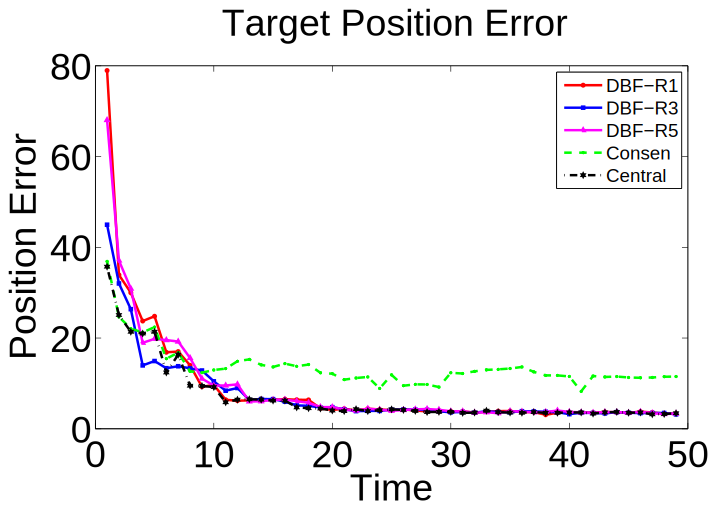
\includegraphics[width=\textwidth]{figures/sta_pos_err.pdf}
%		\caption{Position Error}\label{fig:sta_sen_sta_tar_pos_err}
%	\end{subfigure}
%	\begin{subfigure}[b]{0.23\textwidth}
%		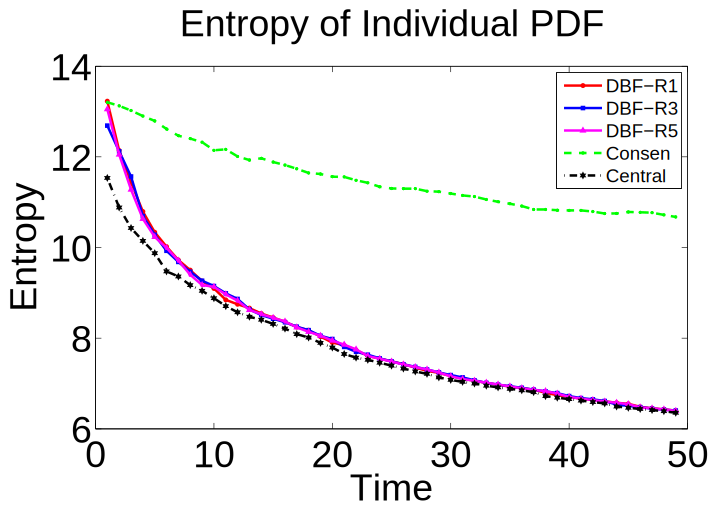
\includegraphics[width=\textwidth]{figures/sta_entropy.pdf}
%		\caption{Entropy of Individual PDF}\label{fig:sta_sen_sta_tar_entropy}
%	\end{subfigure}
%	
%%	\begin{subfigure}[b]{0.4\textwidth}
%%		\includegraphics[width=\textwidth]{figures/sta_sen_sta_tar_30}
%%		\caption{Step 30}\label{fig:sta_sen_sta_tar_all}
%%	\end{subfigure}
%	\caption{(a)-(d) The $1^\text{st}$ UGV's individual PDF at different times. The square denotes the current UGV and stars represent other UGVs. The cross stands for the target. (e) Average position estimation errors of $1^\text{st}$, $3^\text{rd}$ and $5^\text{th}$ UGV's LIFO-DBF, CbDF and CF. (f) Average entropy of individual PDFs.}
%	\label{fig:sta_sen_sta_tar}
%	\vspace{-1.2em}
%\end{figure}

This section simulates a scenario of target localization to evaluate the effectiveness of LIFO-DBF. 
%In all scenarios, each UGV is equipped with a binary sensor. 
The networked UGVs take a ring communication topology that each UGV can communicate with two fixed neighbors.
The probabilistic sensor model
% \cref{eqn:bin_sensor1,eqn:bin_sensor0}, 
takes the form defined in \Cref{eqn:gauss_sensor}.
%which reflects the fact that target detection becomes more probable as the UGV approaches the target position.

The LIFO-DBF is compared with two commonly adopted approaches in multi-agent filtering: the consensus-based distributed filtering (CbDF) method and the centralized filtering (CF) method.
The CbDF requires UGVs to continually exchange their individual PDFs with direct neighbors, computing the average of all received and its own target PDFs. 
Multiple rounds of communication and averaging are conducted at each time step to ensure the convergence of each UGV's individual PDFs.
The CF assumes a central unit that can constantly receive and fuse all UGVs' latest observations into a single PDF.
10 test trials with randomly generated initial target positions are run and each trial is terminated after 50 time steps.
The average error between the estimated and true target position and the average entropy of individual PDFs of all 10 trials are compared. %among these three approaches.

%\subsection{Static UGVs, Static Target}\label{subsec:sim1}
%Six static UGVs, as represented by the green stars and red square in \cref{fig:sta_sen_sta_tar_sing1}, are placed in the field.
%The target is also assumed to be static.
%%, with $A$ being an identity matrix and $B_k$ being a zero matrix in \cref{eqn:tar_motion_model}.
%% shows a test trial when both the UGVs and the target are static. %of the positions of six static UGVs are shown as stars and square.
%%Due to space constraint, only the individual PDF of the first UGV is shown.
%The individual PDF of the first UGV at different time steps are shown in \cref{fig:sta_sen_sta_tar_sing1,fig:sta_sen_sta_tar_sing2,fig:sta_sen_sta_tar_sing3,fig:sta_sen_sta_tar_sing4}.
%%Each UGV constantly receives binary observations of the target.
%%The LIFO-DBF for static target is implemented on each UGV for target localization.
%%The networked UGVs use a ring communication topology that each UGV can communicate with two fixed neighbors.
%%\cref{fig:sta_sen_sta_tar} shows the estimation results of the static target. 
%%After the initial observation, each UGV forms a circular individual PDF, centered at its own position.
%%\cref{fig:sta_sen_sta_tar_sing1} shows the individual PDF after initial observation for $1^\text{st}$ UGV.
%%The circular PDF happens because the Gaussian sensor model (\Cref{eqn:gauss_sensor}) only depends on the distance between UGV and target.
%It can be noticed that, as more measurements are fused, the individual PDF asymptotically concentrates to the true location of the target (\cref{fig:sta_sen_sta_tar_sing4}), which accords with the consistency of LIFO-DBF.
%%In fact, with the Guassian sensor model (\Cref{eqn:gauss_sensor}), all positions with equal distance to a UGV belong to the same equi-parameter set of the UGV.
%%Considering the system of six UGVs located separately, the equi-parameter set that contains the actual target position only contains one element.
%%\cref{fig:entropy} (a) shows the decrease of the entropy of each UGV's individual PDF, indicating the reduction of the uncertainty in PDF estimation.
%
%LIFO-DBF is compared with CbDF and CF, results of which are presented in \cref{fig:sta_sen_sta_tar_pos_err,fig:sta_sen_sta_tar_entropy}\footnote{Since the average estimation errors of all six UGVs' LIFO-DBF are very similar, we only include three UGVs to make figures easier to read.}.
%Unsurprisingly, the CF achieves the best performance in terms of both small position estimation error and fast reduction of entropy. 
%This happens because the central unit has access to the latest observations of all UGVs, thus making most use of all available information.
%It is worth noting that, LIFO-DBF achieves similar asymptotic performance as the CF, both in position estimation error and entropy reduction; this is achieved even though each UGV only communicates with its two neighboring UGVs, which requires less communication burden than the CF.
%The CbDF has the worst performance among these three filtering approaches. 
%It results in slow reduction of entropy and the position error remains large.

%\subsection{Moving UGVs, Moving Target}
\Cref{fig:mov_sen_mov_tar_sing1,fig:mov_sen_mov_tar_sing2,fig:mov_sen_mov_tar_sing3,fig:mov_sen_mov_tar_sing4} shows the evolution of a UGV's individual PDF. %Other five UGVs are represented by the green stars. 
Each UGV moves along a pre-defined circular trajectory.
The target motion is modeled as a single-integrator without process noise.
The LIFO-DBF described in \cref{subsec:LIFO-dbf-mov-tar} is utilized for target localization.
%\cref{fig:mov_sen_mov_tar} shows the estimation results of the moving target. 
It can be noticed that the individual PDF asymptotically concentrates to the true target location. % when the target constantly moves.
%\cref{fig:entropy} (b) shows the decrease of the entropy of the posterior distribution.
\cref{fig:mov_sen_mov_tar_pos_err,fig:mov_sen_mov_tar_entropy} compares LIFO-DBF with CbDF and CF\footnote{Since the average estimation errors of all six UGVs' LIFO-DBF are very similar, we only include three UGVs to make figures easier to read.}.
Unsurprisingly, the CF achieves the best performance in terms of both small position estimation error and fast reduction of entropy. 
This happens because the central unit has access to the latest observations of all UGVs, thus making most use of all available information.
It is worth noting that, LIFO-DBF achieves similar asymptotic performance as the CF, both in position estimation error and entropy reduction; this is achieved even though each UGV only communicates with its two neighboring UGVs. 
%, which requires less communication burden than the CF.
%Similar to results in \cref{subsec:sim1}, CF achieves best performance with smallest position estimation error and fastest entropy reduction; LIFO-DBF shows similar asymptotic performance as the CF; and
CbDF has the slowest entropy reduction among all three filtering approaches.
% but achieves comparable position estimation error as the CF.
%, which are marginally better than LIFO-DBF.
%This is not an unexpected result: due to the consensus procedure, CbDF is able to fuse the latest individual PDFs of each UGV via the averaging process. 
%This is especially useful when the environment is dynamically changing.
%In contrast, LIFO-DBF for each UGV only uses delayed information from neighboring UGVs, thus gaining less knowledge about the target's current position.
We note that CbDF requires multiple rounds of exchanging individual PDFs, which incurs much higher communication burden than LIFO-DBF at each time step.
%'s approach of transmitting the communication buffer once at each time step.
Considering the small difference in position estimation error and significantly faster entropy reduction, LIFO-DBF is preferable over CbDF for moving target scenario.

%\begin{figure}%[thpb]
%	\centering
%	\includegraphics[width=0.5\textwidth]{figures/entropy_all}
%	\caption{Entropy of individual PDFs over time: (a) static UGVs and static target; (b) moving UGVs and moving target.}
%	\label{fig:entropy}
%\end{figure}

\section{CONCLUSION}\label{sec:conclu}
\begin{figure}%[thpb]
	\centering
	\begin{subfigure}[b]{0.21\textwidth}
		\includegraphics[width=\textwidth]{figures/mov_sen_mov_tar_single_6_1}
		\caption{Step 1}\label{fig:mov_sen_mov_tar_sing1}
	\end{subfigure}
	\begin{subfigure}[b]{0.21\textwidth}
		\includegraphics[width=\textwidth]{figures/mov_sen_mov_tar_single_6_5}
		\caption{Step 5}\label{fig:mov_sen_mov_tar_sing2}
	\end{subfigure}	
	\begin{subfigure}[b]{0.21\textwidth}
		\includegraphics[width=\textwidth]{figures/mov_sen_mov_tar_single_6_10}
		\caption{Step 10}\label{fig:mov_sen_mov_tar_sing3}
	\end{subfigure}	
	\begin{subfigure}[b]{0.21\textwidth}
		\includegraphics[width=\textwidth]{figures/mov_sen_mov_tar_single_6_30}
		\caption{Step 30}\label{fig:mov_sen_mov_tar_sing4}
	\end{subfigure}
	\begin{subfigure}[b]{0.21\textwidth}
		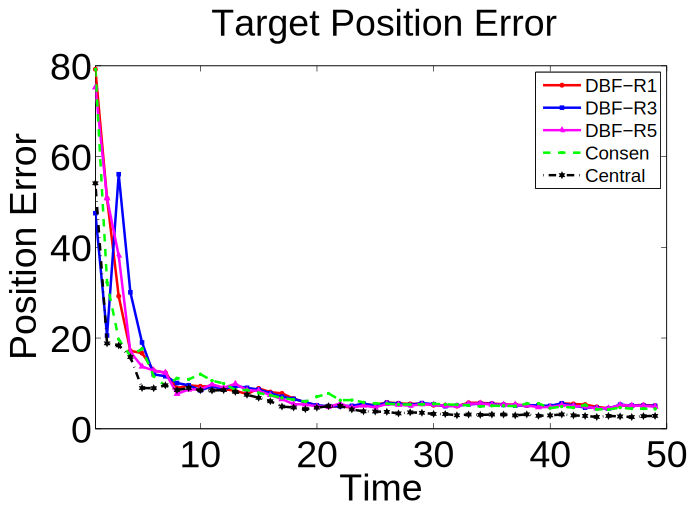
\includegraphics[width=\textwidth]{figures/mov_pos_err.pdf}
		\caption{Position Error}\label{fig:mov_sen_mov_tar_pos_err}
	\end{subfigure}
	\begin{subfigure}[b]{0.21\textwidth}
		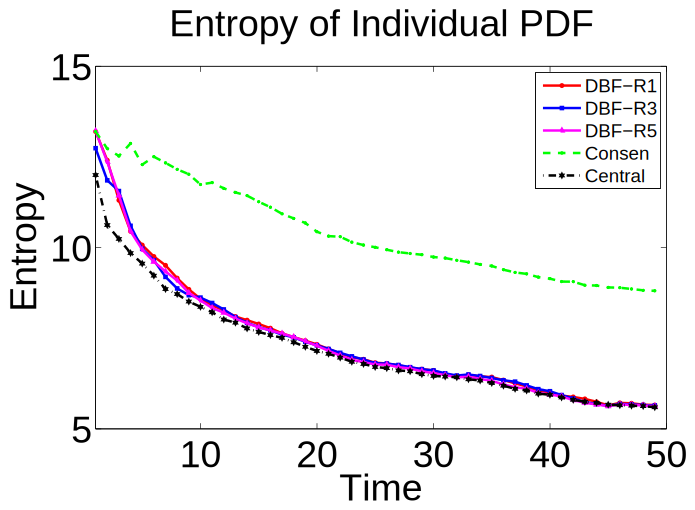
\includegraphics[width=\textwidth]{figures/mov_entropy.pdf}
		\caption{Entropy of PDF}\label{fig:mov_sen_mov_tar_entropy}
	\end{subfigure}
	%	\begin{subfigure}[b]{0.4\textwidth}
	%		\includegraphics[width=\textwidth]{figures/mov_sen_mov_tar_40}
	%		\caption{Step 40}\label{fig:mov_sen_mov_tar_all}
	%	\end{subfigure}
	\caption{(a)-(d) The individual PDF of a UGV (red square) at different times. The stars represent other UGVs. The black cross shows the target position. (e) Average position estimation errors of the $1^\text{st}$, $3^\text{rd}$ and $5^\text{th}$ UGV's LIFO-DBF, CbDF and CF. (f) Average entropy of individual PDFs.}
	\label{fig:mov_sen_mov_tar}
	\vspace{-1.1em}
\end{figure}

This paper presents a measurement dissemination-based distributed Bayesian filtering (DBF) approach for a multi-UGV network, utilizing the Latest-In-and-Full-Out (LIFO) protocol for measurement exchange.
%Different from statistics dissemination approaches that transmit posterior distributions or likelihood functions, each UGV under LIFO only exchanges with neighboring UGVs a full communication buffer consisting of latest available measurements,
%which significantly reduces the transmission burden between each pair of UGVs from the order of environmental size to that of UGV number.
%Under the condition of fixed and undirected topology, LIFO can guarantee non-intermittent dissemination of all observations over the network within finite time via local communication among direct neighborhood.
By exchanging full communication buffers among neighboring UGVs, LIFO significantly reduces the transmission burden between each pair of UGVs. % to scale linearly with the network size.
%, with each UGV non-intermittently receiving observations of all others.
It should be noted that LIFO is a general measurement exchange protocol and thus applicable to various sorts of sensors.
Two types of LIFO-based DBF algorithms are proposed to estimate individual PDFs for a static target and a moving target, respectively and its consistency property is proved.
%by utilizing the law of large numbers, which ensures that the estimated target position converges in probability to the true target position.
Future work includes considering the imperfect communication between UGVs and applying the proposed method for distributed localization and mapping.
%Other types of sensors may have biased measurement, which complicates the design and analysis of LIFO-DBF.
%Imperfect communication, including package loss and transmission delay, requires extensions of current LIFO-DBF approach.

%\addtolength{\textheight}{-12cm}   % This command serves to balance the column lengths
                                  % on the last page of the document manually. It shortens
                                  % the textheight of the last page by a suitable amount.
                                  % This command does not take effect until the next page
                                  % so it should come on the page before the last. Make
                                  % sure that you do not shorten the textheight too much.

%%%%%%%%%%%%%%%%%%%%%%%%%%%%%%%%%%%%%%%%%%%%%%%%%%%%%%%%%%%%%%%%%%%%%%%%%%%%%%%%



%%%%%%%%%%%%%%%%%%%%%%%%%%%%%%%%%%%%%%%%%%%%%%%%%%%%%%%%%%%%%%%%%%%%%%%%%%%%%%%%



%%%%%%%%%%%%%%%%%%%%%%%%%%%%%%%%%%%%%%%%%%%%%%%%%%%%%%%%%%%%%%%%%%%%%%%%%%%%%%%%
%\section*{APPENDIX}
%
%Appendixes should appear before the acknowledgment.

%\section*{ACKNOWLEDGMENT}
%%This work is supported by the Embedded Humans: Provably Correct Decision Making for Networks of Humans and Unmanned Systems project, a MURI project funded by the Office of Naval Research.
%The authors gratefully acknowledges the Office of Naval Research for supporting the research described in this paper. 
%They would also like to thank Yuting Wei in the Department of Statistics, UC Berkeley for her sincere help and fruitful discussion on the consistency proof.

%The preferred spelling of the word �acknowledgment� in America is without an �e� after the �g�. Avoid the stilted expression, �One of us (R. B. G.) thanks . . .�  Instead, try �R. B. G. thanks�. Put sponsor acknowledgments in the unnumbered footnote on the first page.



%%%%%%%%%%%%%%%%%%%%%%%%%%%%%%%%%%%%%%%%%%%%%%%%%%%%%%%%%%%%%%%%%%%%%%%%%%%%%%%%
\bibliographystyle{IEEEtran}
%\bibliographystyle{bibtex}
\bibliography{references}

\end{document}
